%% set up %%%%%%%%%%%%%%%%%%%%%%%%%%%%%%%%%%%%%%%%%%%%%%%%%%%%%%%%%%%%%%%%%%%%%%
\documentclass[article]{jss}
\usepackage{amstext}
\usepackage{amsmath}
\usepackage{graphicx}
\usepackage{natbib}


%% declarations for jss.cls %%%%%%%%%%%%%%%%%%%%%%%%%%%%%%%%%%%%%%%%%%%%%%%%%%%%
\author{Timothy D. Meehan\\National\\Audubon Society \And
        Nicole L. Michel\\National\\Audubon Society \And
        H\"{a}vard Rue\\King Abdulla University\\of Science and Technology}
\title{Estimating Animal Abundance with N-Mixture Models Using the \pkg{R-INLA} Package for R}

%% for pretty printing
%% comma-separated
\Plainauthor{Timothy D. Meehan, Nicole L. Michel, H\"{a}vard Rue}
%% without formatting
\Plaintitle{Estimating Animal Abundance with N-Mixture Models Using the R-INLA Package for R}
%% a short title
\Shorttitle{\pkg{R-INLA} for N-Mixture Models}

%% an abstract and keywords
\Abstract{
  Successful management of wildlife populations requires accurate estimates of abundance.  Abundance estimates can be confounded by imperfect detection during wildlife surveys. Development of N-mixture models has facilitated quantification of detectability and has improved our ability to produce accurate abundance estimates. The purpose of this study was to demonstrate the use of the \pkg{R-INLA} package to analyze N-mixture models and to compare performance of \pkg{R-INLA} to two other common approaches -- \proglang{JAGS} (via the \pkg{runjags} package), which uses Markov chain Monte Carlo methods and allows Bayesian inference, and \pkg{unmarked}, which uses Maximum Likelihood and allows Frequentist inference. Our results suggest that \pkg{R-INLA} is an attractive option for analyzing N-mixture models when (1) survey level covariates are not essential, (2) familiar model syntax and data format are desired (relative to other R packages), (3) fast computing time is necessary (\pkg{R-INLA} is 10 times faster than \pkg{unmarked}, 300 times faster than \proglang{JAGS}), and (4) Bayesian inference is preferred.

}
\Keywords{wildlife, abundance, detection, N-mixture models, \pkg{R-INLA}, \proglang{R}, \proglang{BUGS}}
%% without formatting
\Plainkeywords{wildlife, abundance, detection, N-mixture models, R-INLA, R, BUGS}

%% publication information
%% NOTE: This can be left commented and will be filled out by the technical editor
%% \Volume{50}
%% \Issue{9}
%% \Month{June}
%% \Year{2012}
%% \Submitdate{2012-06-04}
%% \Acceptdate{2012-06-04}

%% The address of (at least) one author should be given
\Address{
  Timothy D. Meehan\\
  National Audubon Society\\
  Boulder, Colorado USA\\
  E-mail: \email{tmeehan@audubon.org}\\
\\
  Nicole L. Michel\\
  National Audubon Society\\
  San Francisco, California USA\\
  E-mail: \email{nmichel@audubon.org}\\
  \\
  H\"{a}vard Rue\\
  King Abdulla University
  of Science and Technology\\
  Thuwal, SAU\\
  E-mail: \email{haavard.rue@kaust.edu.sa }
}
%% end of declarations %%%%%%%%%%%%%%%%%%%%%%%%%%%%%%%%%%%%%%%%%%%%%%%%%%%%%%%%%



%% start main document %%%%%%%%%%%%%%%%%%%%%%%%%%%%%%%%%%%%%%%%%%%%%%%%%%%%%%%%%
\begin{document}

%% introduction
\section[Introduction]{Introduction}
\subsection[Background]{Background}
Successful management of wildlife species requires accurate estimates of abundance \citep{Yoccoz_Nichols_Boulinier_2001}.  One common method for estimating animal abundance is direct counts \citep{Pollock_Nichols_Simons_Farnsworth_Bailey_Sauer_2002}.  Efforts to obtain accurate abundance estimates via direct counts can be hindered by both the cryptic nature of many wildlife species and by other factors such as observer expertise, weather, and habitat structure.  The lack of perfect detection in wildlife surveys is common, and can cause abundance to be greatly underestimated \citep{Wenger_Freeman_2008, Joseph_Elkin_Martin_Possingham_2009}.

In recent years, new sampling schemes and modeling approaches have enabled improved estimates of animal abundance that are less biased by non-detection \citep{Denes_Silveira_Beissinger_2015}.  One such sampling scheme, termed a "metapopulation design" \citep{Kery_Royle_2010}, involves repeat visits in rapid succession to each of multiple study sites in a study area.  If, during repeat visits, the population is assumed to be closed (no immigration , emigration, or reproduction), then the ratio of detections to non-detections during repeated counts can inform an estimate of detection probability.  This detection probability can, in effect, be used to correct abundance estimates for imperfect detection \citep{Denes_Silveira_Beissinger_2015}.

Data resulting from this sampling scheme are often modeled using an explicitly hierarchical statistical model referred to as an N-mixture model \citep{Royle_Nichols_2003, Dodd_Dorazio_2004, Royle_2004, Kery_Royle_Schmid_2005}.  A simple form of an N-mixture model, a binomial mixture model, describes observed counts $Y$ at site $i$ during survey $j$ as coming from a binomial distribution with parameters for abundance $N$ and detection probability $p$, where $N$ per site is drawn from a Poisson distribution with an expected value, lambda $(\lambda)$. Specifically,

$$N_i \sim \text{Poisson}(\lambda) \qquad \text{and} \qquad  Y_{i,j} | N_i \sim \text{binomial}(N_i, p).$$

$\lambda$ is commonly modeled as a log-linear function of site covariates, as $\text{log}(\lambda_i) = \beta_0 + \beta_1 * x_i$. Similarly, $p$ is commonly modeled as $\text{logit}(p_{i,j}) = \alpha_0 + \alpha_1 * x_{i,j}$, a logit-linear function of site-survey covariates.

This estimation approach can be extended to cover $K$ distinct breeding seasons, which correspond with distinct years for annually-breeding wildlife species \citep{Kery_Dorazio_Soldaat_Van_Strien_Zuiderwijk_Royle_2009}.  In this case, population closure is assumed across $J$ surveys within year $k$, but is relaxed across years \citep{Kery_Dorazio_Soldaat_Van_Strien_Zuiderwijk_Royle_2009}. A simple specification of a multiple-year model is $N_{i,k} \sim \text{Poisson}(\lambda_{i,k}), \quad Y_{i,j,k} | N_{i,k} \sim \text{binomial}(N_{i,k}, p_{i,k})$.  Like the single-year specification, $\lambda$ is commonly modeled using site and site-year covariates, and $p$ using site-survey-year covariates.  There are other variations of N-mixture models that accommodate overdispersed counts through use of a negative binomial distribution \citep{Kery_Royle_2010}, zero-inflated Poisson distribution \citep{Wenger_Freeman_2008}, or survey-level random intercepts \citep{Kery_Schaub_2011}.  Yet other variations account for non-independent detection probabilities through use of a beta-binomial distribution \citep{Martin_Royle_Mackenzie_Edwards_Kery_Gardner_2011}, parse different components of detection through the use of unique covariates \citep{O'Donnell_Thompson_III_Semlitsch_2015}, or relax assumptions of population closure \citep{Chandler_Royle_King_2011, Dail_Madsen_2011}.  We do not discuss all of these variations here, but refer interested readers to \cite{Denes_Silveira_Beissinger_2015} for a nice overview.

The development of metapopulation designs and N-mixture models represents a significant advance in quantitative wildlife ecology.  However, there are practical issues that sometimes act as barriers to adoption.  Much of the development of N-mixture models, and many of the examples in the wildlife literature, implement models using Bayesian modeling software such as \proglang{WinBUGS}, \proglang{OpenBUGS}, or \proglang{JAGS} \citep{Lunn_Jackson_Best_Thomas_Spiegelhalter_2012}.  These are extremely powerful and flexible platforms for analyzing Bayesian models, but they come with a few important challenges.  First, many wildlife biologists are not accustomed to coding statistical models using the \proglang{BUGS} modeling syntax.  While there are several outstanding resources aimed at teaching this skill \citep{Royle_Dorazio_2008, Kery_2010, Kery_Schaub_2011, Kery_Royle_2015} it is, nonetheless, a considerable commitment.  Second, while Markov chain Monte Carlo (MCMC) chains converge quickly for relatively simple N-mixture models, convergence for more complex models can take hours to days, and may not occur at all.

There are other tools available for analyzing N-mixture models that alleviate some of these practical issues.  The \pkg{unmarked} package \citep{Fiske_Chandler_others_2011} for \proglang{R} statistical computing software \citep{R_Core_Team_2016} offers several options for analyzing N-mixture models within a Frequentist framework, with the capacity to accommodate overdispersion and dynamic populations.  The model coding syntax used in \pkg{unmarked} is a simple extension of the standard \proglang{R} syntax.  Models are analyzed using a Maximum Likelihood (ML), so model analysis is often completed in a fraction of the time taken using an MCMC approach.  The familiar model syntax and rapid model evaluation of \pkg{unmarked} has undoubtedly contributed to the broader adoption of N-mixture models by wildlife biologists.  However, it comes at a cost -- the loss of the intuitive inferential framework associated with Bayesian analysis.

Here we discuss analysis of N-mixture models using the \pkg{R-INLA} package \citep{Rue_Martino_Lindgren_Simpson_Riebler_2013} for \proglang{R}.  The \pkg{R-INLA} package uses integrated nested Laplace approximation (INLA) to derive posterior distributions for a large class of Bayesian statistical models that can be formulated as latent Gaussian models \citep{Rue_Martino_Chopin_2009}. INLA was developed to allow estimation of posterior distributions in a fraction of the time taken by MCMC.  Like \pkg{unmarked}, the model syntax used in the \pkg{R-INLA} package is a straightforward extension of the modeling syntax commonly used in R.  Also, like \pkg{unmarked}, the computational cost of analyzing models with \pkg{R-INLA} is relatively low.  The \pkg{R-INLA} approach is different from \pkg{unmarked} in that inference about model parameters falls within a Bayesian framework.

\subsection[Overall objectives]{Overall objectives}
The purpose of this manuscript is to demonstrate analysis of N-mixture models using the \pkg{R-INLA} package. In the process, we employ simulated and real count datasets, and analyze them using \proglang{JAGS}, via the \pkg{runjags} package \citep{Denwood_2016} for \proglang{R}, the \pkg{unmarked} package, and the \pkg{R-INLA} package. In each case, we demonstrate how data are formatted, how models are specified, how model estimates compare to simulation inputs, and how methods compare in terms of computational performance. We also explore a limitation of the \pkg{R-INLA} approach related to model specification.  Specifically, while it is possible to specify survey level covariates for detection using \proglang{JAGS} and \pkg{unmarked}, this is not possible using \pkg{R-INLA}.  Rather, survey level covariates of detection must be averaged to the site or site-year level.  Using an averaged detection covariate does allow accounting for site-level differences in survey conditions should they occur.  However, in the process of averaging, important information related to detection is discarded, which could lead to biased detection and abundance estimates under certain conditions.

Much of the code used to conduct analyses is shown in the body of this manuscript. However, some repeated code, and code related to generating tables and figures, is not shown for brevity.  All code can be accessed via \url{https://github.com/tmeeha/inlaNMix}.

\subsection[Simulated data]{Simulated data}
The data simulated for this analysis were intended to represent a typical wildlife study. To put the simulation in context, consider an effort to estimate the abundance of a bird species in a national park, within which are located 72 study sites. At each site, 3 replicate surveys are conducted within 6 weeks, during the peak of the breeding season when birds are likely to be singing. In order to estimate a trend in abundance over time, these repeated surveys are conducted over a 9-year period.

In this scenario, the abundance of the species is thought to vary with two site-level covariates ($\lambda$ covariates 1 and 2) that represent habitat characteristics at a site and do not change appreciably over time. The detection probability is also believed to vary according to two covariates ($p$ covariates 1 and 3). The first covariate for detection, $p$ covariate 1, is the same site-level covariate 1 that affects abundance, although it has the opposite effect on detection. The other detection covariate, $p$ covariate 3, is a site-survey-year variable that could be related to weather conditions during an individual survey.

As is commonly the case, we assume that the counts are overdispersed due to the effects of unknown variables. Overdispersion was generated and modeled using a negative binomial distribution for the count component of the model. The specific model parameters and their simulated values were: p.b0 = 1.0 ($p$ intercept), p.b1 = -2.0 (effect of $p$ covariate 1), p.b3 = 1.0 (effect of $p$ covariate 3), lam.b0 = 2.0 ($\lambda$ intercept), lam.b1 = 2.0 (effect of $\lambda$ covariate 1), lam.b2 = -3.0 (effect of $\lambda$ covariate 2), lam.b4 = 1.0 (effect of year on $\lambda$), disp.size = 3.0 (size of the overdispersion parameter). All independent variables in the simulation were centered at zero to alleviate computational difficulties and to make model intercepts more easily interpreted.

We simulated data for this study using the following function.  Note that the function produces two versions of detection covariate 3, x.p.3 and x.p.3.mean, and two versions of the count matrix, y1 and y2.  x.p.3 is the site-survey-year variable described above.  It is used to generate y2, which is used in Example II.  x.p.3.mean is derived from x.p.3, where values are unique to site and year, but averaged over surveys.  It is used to generate y1, which is used in Example I.

\begin{Code}
R> data4sim <- function(n.sites = 72,   # number study sites
+                       n.surveys = 3,  # short term replicates
+                       n.years = 9,    # number years
+                       lam.b0 = 2.0,   # intercept for log lambda
+                       lam.b1 = 2.0,   # slope for log lambda cov 1
+                       lam.b2 = -3.0,  # slope for log lambda cov 2
+                       lam.b4 = 1.0,   # slope for log lambda year
+                       p.b0 = 1.0,     # intercept for logit p
+                       p.b1 = -2.0,    # slope for logit p cov 1
+                       p.b3 = 1.0,     # slope for logit p cov 3
+                       disp.size = 3.0 # size of overdispersion
+                       ){
+  # setup
+  if(n.years %% 2 == 0) {n.years <- n.years + 1}     # make years odd
+  N.tr <- array(dim = c(n.sites, n.years))           # for abund
+  y1 <- array(dim = c(n.sites, n.surveys, n.years))  # for ex1 counts
+  y2 <- array(dim = c(n.sites, n.surveys, n.years))  # for ex2 counts
+  # abundance covariate values
+  x.lam.1 <- array(as.numeric(scale(runif(n = n.sites, -0.5, 0.5), 
+                   scale = F)), dim = c(n.sites, n.years))
+  x.lam.2 <- array(as.numeric(scale(runif(n = n.sites, -0.5, 0.5), 
+                   scale = F)), dim = c(n.sites, n.years))
+  yrs <- 1:n.years
+  yrs <- (yrs - mean(yrs)) / (max(yrs - mean(yrs))) / 2
+  yr <- array(rep(yrs, each = n.sites), dim = c(n.sites, n.years))
+  # fill abundance array
+  lam.tr <- exp(lam.b0 + lam.b1*x.lam.1 + lam.b2*x.lam.2 + lam.b4*yr)
+  for(i in 1:n.sites){
+    for(k in 1:n.years){
+    N.tr[i, k] <- rnbinom(n = 1, mu = lam.tr[i, k], size = disp.size)
+  }}
+  # detection covariate values
+  x.p.1 <- array(x.lam.1[,1], dim = c(n.sites, n.surveys, n.years))
+  x.p.3 <- array(as.numeric(scale(runif(n = n.sites*n.surveys*n.years, 
+                                        -0.5, 0.5), scale=F)), 
+                 dim=c(n.sites, n.surveys, n.years))
+  # average x.p.3 per site-year
+  x.p.3.mean <- apply(x.p.3, c(1,3), mean, na.rm=F)
+  out1 <- c()
+  for(k in 1:n.years){
+   chunk1 <- x.p.3.mean[,k]
+   chunk2 <- rep(chunk1, n.surveys)
+   out1 <- c(out1, chunk2)
+  }
+  x.p.3.arr <- array(out1, dim=c(n.sites, n.surveys, n.years))
+  # fill count array with site-yr x.p.3
+  p.tr1 <- plogis(p.b0 + p.b1*x.p.1 + p.b3*x.p.3.arr)
+  for (i in 1:n.sites){
+    for (k in 1:n.years){
+      for (j in 1:n.surveys){
+        y1[i,j,k] <- rbinom(1, size = N.tr[i,k], prob = p.tr1[i,j,k])
+  }}}
+  # fill count array with site-surv-yr x.p.3
+  p.tr2 <- plogis(p.b0 + p.b1 * x.p.1 + p.b3 * x.p.3)
+  for (i in 1:n.sites){
+    for (k in 1:n.years){
+      for (j in 1:n.surveys){
+        y2[i,j,k] <- rbinom(1, size = N.tr[i,k], prob = p.tr2[i,j,k])
+  }}}
+  # return data
+  return(list(n.sites = n.sites, n.surveys = n.surveys, n.years = n.years,
+              x.p.1 = x.p.1[,1,1], x.p.3 = x.p.3, x.p.3.mean = x.p.3.mean,
+              x.p.3.arr = x.p.3.arr, x.lam.1 = x.lam.1[,1],
+              x.lam.2 = x.lam.2[,1], yr = yr[1,], y1 = y1, y2 = y2,
+              lam.tr = lam.tr, N.tr = N.tr))
+  } #end function
R> set.seed(12345) # make results reproducible
R> sim.data <- data4sim() # create datasets
\end{Code}

\subsection[Real data]{Real data}
In addition to simulated data, we also demonstrate the use of \pkg{R-INLA} with a real dataset in Example III.  This dataset comes from a study by \cite{Kery_Royle_Schmid_2005} and is publicly available as part of the \pkg{unmarked} package.  The dataset includes mallard duck (\emph{Anas platyrhynchos}) counts, conducted at 239 sites on 2 or 3 occasions during the summer of 2002 as part of a Swiss program that monitors breeding bird abundance (Monitoring H\"{a}ufige Brutv\"{o}gel). In addition to counts, the dataset also includes 2 site-survey covariates related to detection (survey effort and survey date), and 3 site level covariates related to abundance (route length, elevation, and forest cover).  Full dataset details are given in \cite{Kery_Royle_Schmid_2005}.

%% example 1
\section[Example I]{Example I}
\subsection[Goals]{Goals}
In Example I, we demonstrate the use of \pkg{R-INLA} and compare use and performance to similar analyses using \proglang{JAGS} and \pkg{unmarked}.  In this exercise, the functional forms of \proglang{JAGS}, \pkg{unmarked}, and \pkg{R-INLA} models match the data generating process.  Specifically, we used the covariate x.p.3.mean to generate the count matrix y1 and analyzed the data with models that use x.p.3.mean as a covariate.  This exercise was intended to demonstrate the differences and similarities in use, computation time, and estimation results across the three packages when the specified model was reasonably close to the data generating process.

\subsection[Analysis with JAGS]{Analysis with JAGS}
We first analyzed the simulated data using \proglang{JAGS}, via the \pkg{runjags} package. In defining the model, we specified a negative binomial distribution for the abundance component, and used vague normal priors for the intercepts and the global effects of the covariates of $\lambda$ and $p$.

\begin{Code}
R> jags.model.string <- "
+    model {
+    # priors
+    intP ~ dnorm(0, 0.01)       # detection intercept
+    bCov1P ~ dnorm(0, 0.01)     # detection cov 1 effect
+    bCov3P ~ dnorm(0, 0.01)     # detection cov 3 effect
+    intLam ~ dnorm(0, 0.01)     # lambda intercept
+    bCov1Lam ~ dnorm(0, 0.01)   # lambda cov 1 effect
+    bCov2Lam ~ dnorm(0, 0.01)   # lambda cov 2 effect
+    bYr ~ dnorm(0, 0.01)        # year effect
+    overDisEst ~ dunif(0, 5)    # overdispersion size
+    # abundance component
+    for (k in 1:nYears){
+      for (i in 1:nSites){
+        N[i, k] ~ dnegbin(prob[i, k], overDisEst) # negative binomial specification
+        prob[i, k] <- overDisEst / (overDisEst + lambda[i, k]) # overdispersion effect
+        log(lambda[i, k]) <- intLam + (bCov1Lam * x.lam.1[i]) + (bCov2Lam * x.lam.2[i]) +
+                          (bYr * yr[k])
+    # detection component
+        for (j in 1:nSurveys){
+          y[i, j, k] ~ dbin(p[i,j,k], N[i,k])
+          p[i, j, k] <- exp(lp[i,j,k]) / (1 + exp(lp[i,j,k]))
+          lp[i, j, k] <- intP + (bCov1P * x.p.1[i]) + (bCov3P * x.p.3[i, k])
+        } # close j loop
+      } # close i loop
+    } # close k loop
+  } # close model loop
+  "
\end{Code}

Next, we defined the parameters to be monitored during the MCMC runs, bundled the data for \proglang{JAGS}, and created a function for drawing random initial values for the model parameters.  The initial values for abundance were made to avoid values of "NA" and zero, as these would cause computational problems.

\begin{Code}

R> params <- c("intP", "bCov1P", "bCov3P", "intLam", "bCov1Lam","bCov2Lam",
+              "bYr", "overDisEst") # parameters to monitor
R> jags.data <- list(y = sim.data$y1, x.lam.1 = sim.data$x.lam.1,
+               x.lam.2 = sim.data$x.lam.2, yr = sim.data$yr,
+               x.p.1 = sim.data$x.p.1, x.p.3 = sim.data$x.p.3.mean,
+               nSites = sim.data$n.sites, nSurveys = sim.data$n.surveys,
+               nYears = sim.data$n.years)
R> N.init <- sim.data$y1 # initial count values
R> N.init[is.na(N.init)] <- 1 # clean up NA's
R> N.init <- apply(N.init, c(1, 3), max) + 1 # zero values cause trouble
R> inits <- function() list(N = N.init, intLam = rnorm(1, 0, 0.01),
+                      intP = rnorm(1, 0, 0.01), bCov1P = rnorm(1, 0, 0.01),
+                      bCov2Lam = rnorm(1,0,0.01), bCov1Lam = rnorm(1, 0, 0.01),
+                      bCov3P = rnorm(1, 0, 0.01), bYr = rnorm(1, 0, 0.01),
+                      overDisEst = runif(1, 0.5, 2.5))
\end{Code}

Finally, we set the run parameters and started the MCMC process. Run parameters were chosen such that MCMC diagnostics indicated converged chains (Gelman-Rubin statistics < 1.05) and reasonably robust posterior distributions (effective sample sizes > 1000).  Note that the recommended number of effective samples for particularly robust inference is closer to 6000 \citep{Gong_Flegal_2016}.  So MCMC processing times reported here could be considered low estimates.

\begin{Code}
R> nc <- 3; na <- 2500; nb <- 2500; ni <- 5000; nt <- 10 # set run parameters
R> out.jags <- run.jags(model = jags.model.string, data = jags.data,
+                       monitor = params, n.chains = nc, inits = inits,
+                       burnin = nb, adapt = na, sample = ni, thin = nt,
+                       modules = "glm on", method = "parallel")
\end{Code}

Mean parameter estimates from the \proglang{JAGS} model were reasonably close to, and not significantly different from, the input values used to generate the data (Fig. \ref{fig:fig1}).  The potential scale reduction factor for all variables was < 1.01, and the effective sample size for all variables was > 2410.  The simulation ran in parallel on 3 virtual cores, 1 MCMC chain per core, and took approximately 2104 seconds.

%% figure 1
\begin{figure}
  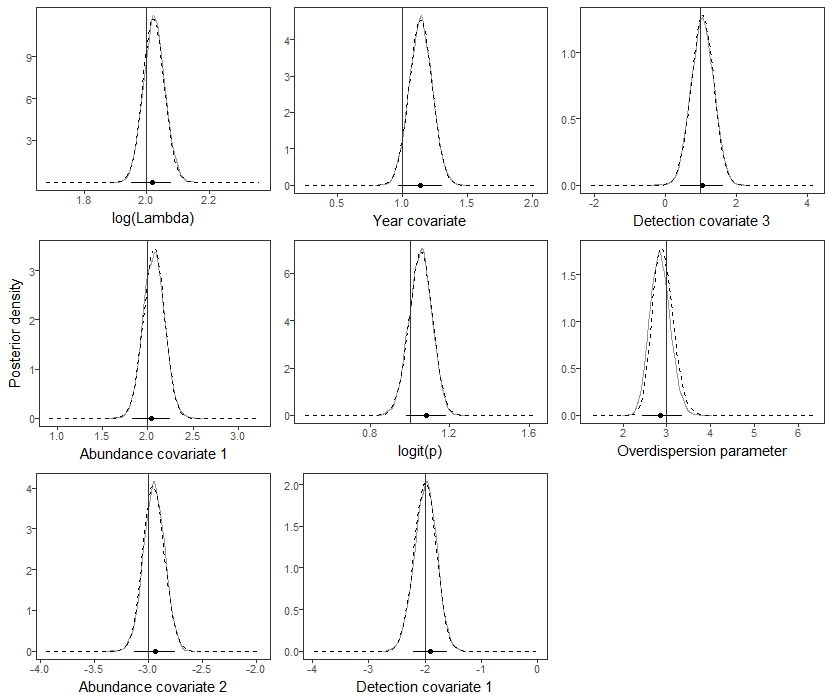
\includegraphics[width=\linewidth]{fig1.jpeg}
  \caption{Marginal posteriors from \proglang{JAGS} (solid gray lines) and \pkg{R-INLA} (dashed black lines), along with Maximum Liklihood estimates (black circles) and 95\% confidence intervals (horizontal black lines) from \pkg{unmarked}.  True input values are represented by vertical black lines.}
  \label{fig:fig1}
\end{figure}
%% end figure 1

\subsection[Analysis with unmarked]{Analysis with unmarked}
Next, we prepared the simulated data for the \pkg{unmarked} analysis, which involved slight modification of the data in the sim.data object.  Here, the count data was changed from a 3-dimensional $I*J*K$ array to a 2-dimensional $I*K$ row by $J$ column matrix.  Each static site level variable was duplicated and stacked $K$ times to form a single-column vector. A column vector was created to identify each year in the stacked data.  The site-year variable, x.p.3.mean, was transformed from 2-dimensional matrix to a single column vector.  Reformatted variables were then assembled in an \pkg{unmarked} data structure called an unmarked frame.

\begin{Code}
R> y.unmk <- sim.data$y1[ , , 1]
R> for(i in 2:sim.data$n.years){
+    y.chunk <- sim.data$y1[ , , i]
+    y.unmk <- rbind(y.unmk, y.chunk)
+  } 
R> x.lam.1.unmk <- rep(sim.data$x.lam.1, sim.data$n.years)
R> x.lam.2.unmk <- rep(sim.data$x.lam.2, sim.data$n.years)
R> yr.unmk <- rep(sim.data$yr, each = sim.data$n.sites)
R> x.p.1.unmk <- rep(sim.data$x.p.1, sim.data$n.years)
R> x.p.3.unmk <- c(sim.data$x.p.3.mean)
R> site.covs.unmk <- data.frame(x.lam.1.unmk, x.lam.2.unmk, yr.unmk,
+                               x.p.1.unmk, x.p.3.unmk)
R> unmk.data <- unmarkedFramePCount(y = y.unmk, siteCovs = site.covs.unmk)
\end{Code}

The first argument in the call to the pcount() function was the model formula, which specified the covariates for detection and then the covariates for abundance.  This was followed by an argument identifying the appropriate unmarked frame, and the form of the mixture model, negative binomial-binomial.

\begin{Code}
R> out.unmk <- pcount(~ x.p.1.unmk + x.p.3.unmk
+                     ~ x.lam.1.unmk + x.lam.2.unmk + yr.unmk,
+                     data = unmk.data, mixture = "NB")
\end{Code}

Maximum likelihood estimates from the \pkg{unmarked} analysis are also close to, and not significantly different from, input values (Fig. \ref{fig:fig1})  The \pkg{unmarked} estimates were produced in approximately 77 seconds.

\subsection[Analysis with R-INLA]{Analysis with R-INLA}
Next, we prepared data for \pkg{R-INLA}, which uses data formats similar to those used by \pkg{unmarked}. The object counts.and.count.covs is an \pkg{R-INLA} object that includes an $I*K$ row by $J$ column matrix of counts. Next comes a value of 1, which is turned into an $I*K$ length vector of ones to specify that the model has a global intercept for $\lambda$. Finally, there are two $I*K$ length vector of values for the two static site covariates of abundance, where the vector of values for $I$ sites is stacked $K$ times.  In addition to the counts.and.count.covs object, we also defined x.p.1.inla, which is a copy of x.lam.1.inla, and x.p.3.inla, which is the $I*K$ length vector corresponding with x.p.3.mean.

\begin{Code}

R> y.inla <- sim.data$y1[ , , 1]
R> for(i in 2:sim.data$n.years){
+    y.chunk <- sim.data$y1[ , , i]
+    y.inla <- rbind(y.inla, y.chunk)
+  }
R> x.lam.1.inla <- rep(sim.data$x.lam.1, sim.data$n.years)
R> x.lam.2.inla <- rep(sim.data$x.lam.2, sim.data$n.years)
R> yr.inla <- rep(sim.data$yr, each = sim.data$n.sites)
R> x.p.1.inla <- rep(sim.data$x.p.1, sim.data$n.years)
R> x.p.3.inla <- c(sim.data$x.p.3.mean)
R> counts.and.count.covs <- inla.mdata(y.inla, 1, x.lam.1.inla, 
+                                      x.lam.2.inla, yr.inla)
\end{Code}

The call to the inla() function includes several components.  First is the model statement.  On the left side of the formula is the counts.and.count.covs object that includes the matrix of counts and the covariates related to $\lambda$.  On the right side of the formula is a 1 to specify a global intercept for $p$ and the two fixed covariates for $p$.  Note that a wide range of random effects for $p$ could be added to the right side of the formula \citep{Rue_Martino_Lindgren_Simpson_Riebler_2013}.  The second argument describes the data, provided here as a list that corresponds with the model formula.  Third is the likelihood family, which can take values of "nmix" for a Poisson-binomial mixture and "nmixnb" for a negative binomial-binomial mixture.  The fourth and fifth arguments specify the priors for the two model components.  In this case, the priors are specified similarly to those in the \proglang{JAGS} model, but a variety of other options are available. Several other characteristics of the analysis can be modified using the call to inla().  See \cite{Rue_Martino_Lindgren_Simpson_Riebler_2013} for details.

\begin{Code}
R> out.inla <- inla(counts.and.count.covs ~ 1 + x.p.1.inla + x.p.3.inla,
+           data = list(counts.and.count.covs = counts.and.count.covs,
+                       x.p.1.inla = x.p.1.inla, x.p.3.inla = x.p.3.inla),
+           family = "nmixnb",
+           control.fixed = list(mean = 0, mean.intercept = 0, prec = 0.01,
+                                prec.intercept = 0.01),
+           control.family = list(hyper = list(theta1 = list(param = c(0, 0.01)),
+                                              theta2 = list(param = c(0, 0.01)),
+                                              theta3 = list(param = c(0, 0.01)),
+                                              theta4 = list(param = c(0, 0.01)),
+                                              theta5 = list(prior = "flat",
+                                                            param = numeric()))))
\end{Code}

Mean parameter estimates from the \pkg{R-INLA} model are also close to, and not significantly different from, input values (Fig. \ref{fig:fig1})  Full marginal posterior distributions from \pkg{R-INLA} are shown in Fig. \ref{fig:fig1}.  The analysis took approximately 6 seconds.

\subsection[Example I summary]{Example I summary}
Example I demonstrated basic use of \pkg{R-INLA} and highlighted similarities and differences between it and two other commonly used approaches.  In demonstrating the use of \pkg{R-INLA}, we show that the input data format is not complicated, and that the formatting process can be accomplished with relatively few lines of code.  Similarly, model specification uses a straightforward extension of the standard syntax in R, where the count matrix and covariates for $\lambda$ are specified through an \pkg{R-INLA} object included on the left side of the formula, and covariates for $p$ are specified on the right side of the formula. Data format and model specification syntax of \pkg{R-INLA} are not too different from \pkg{unmarked}, which are both considerably different from \proglang{JAGS} and other \proglang{BUGS}-oriented MCMC software.

Regarding performance, \pkg{R-INLA}, \pkg{unmarked}, and \proglang{JAGS} successfully extracted simulation input values.  Fig. \ref{fig:fig1} depicts marginal posterior distributions produced by \proglang{JAGS} and \pkg{R-INLA}, and 95\% confidence intervals from \pkg{unmarked}.   These results derive from data resulting from one random manifestation of the input values.  Thus, we do not expect the posterior distributions for the estimates to be centered at the input values, which would be expected if the simulation was repeated many times.  However, we do expect the input values to fall somewhere within the posterior distributions and 95\% confidence intervals, which is what occurs here.  Fig. \ref{fig:fig1} shows that, for similarly specified models, \pkg{R-INLA} (dashed black lines) and \proglang{JAGS} (solid gray lines) yielded practically identical marginal posterior distributions for model parameters.

Where \pkg{R-INLA}, \pkg{unmarked}, and \proglang{JAGS} differed was in computing time.  In this example, \pkg{R-INLA} took 6 seconds, \pkg{unmarked} took 77 seconds, and \proglang{JAGS} took 2104 seconds to produce results. Thus, \pkg{R-INLA} was approximately 10 times faster than \pkg{unmarked} and 300 times faster than \proglang{JAGS}.  This was the case despite the fact that \pkg{unmarked} uses ML algorithms and the \proglang{JAGS} model was run in parallel with each of three MCMC chains simulated on a separate virtual computing core.  If parallel computing had not been used with \proglang{JAGS}, processing the \proglang{JAGS} model would have taken approximately twice as long.  If MCMC simulations were run until an effective sample size of 6000 was reached, processing times would have doubled again.

In sum, when compared to other tools, \pkg{R-INLA} is relatively easy to implement and produces accurate estimates of Bayesian posteriors very quickly. Its utility depends on the degree to which the data generating process can be captured accurately in model specification.  However, as mentioned above, certain models can not be specified using \pkg{R-INLA}.  For the data in Example I, the count matrix was produced using a detection covariate that was averaged to the site-year level.  This averaged covariate was subsequently used in the analysis. But what happens when the site-survey-year covariate is an important component of the data generating process, and it can't be specified in the model in this form?  This is the question explored in Example II.

%% example 2
\section[Example II]{Example II}
\subsection[Goals]{Goals}
In Example 2, we show the consequences of not being able to specify a site-survey-year covariate under a range of conditions.  Specifically, we conducted a Monte Carlo simulation where, for each iteration, the count matrix for the analysis, y2, was generated with the data generating function described in 1.3, using the site-survey-year covariate x.p.3.  The count data were then analyzed with two \proglang{JAGS} models.  One model incorporated an averaged site-survey x.p.3.mean as a covariate, such as in 2.1.  The other model incorporated the site-survey-year covariate instead.  In each iteration we randomly varied the size of the effect for x.p.3.  We suspected that the simpler model, with x.p.3.mean, would yield biased estimates when the effect of x.p.3 was relatively large, and unbiased estimates when the effect was relatively small.

\subsection[Analysis with JAGS]{Analysis with JAGS}
Given the long processing time associated with \proglang{JAGS} models, we only ran 3000 iterations (after 1000 adaptive iterations and 1000 burn-in iterations) during each simulation.  This number is not sufficient for drawing inference from marginal posteriors, but was sufficient for looking at qualitative patterns in posterior means.  In each of the 50 iterations the size of the effect for x.p.3 was drawn from a uniform distribution that ranged from -3 to 3. The results of the simulations are depicted in Fig. \ref{fig:fig2}.

%% figure 2
\begin{figure}
  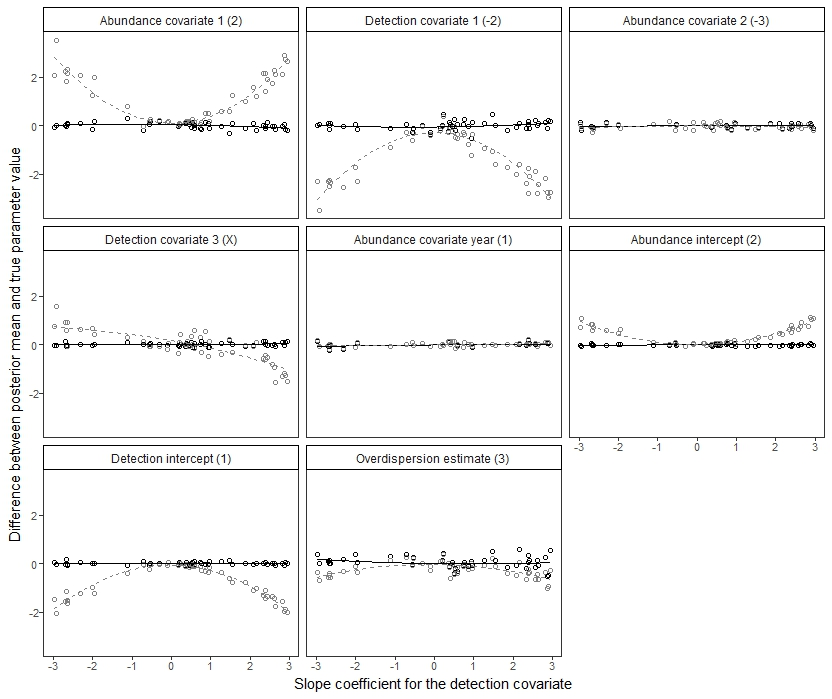
\includegraphics[width=\linewidth]{fig2.jpeg}
  \caption{Differences between the estimated posterior mean values and the true input parameter values as a function of the slope coefficient (effect size) for the site-survey-year covariate, x.p.3.  Black circles and lines are output from the model with the site-survey-year covariate, x.p.3, and gray circles and lines are from the model with an averaged site-year covariate, x.p.3.mean.  Parameter name and true input value is given in the strip across the top of each panel.}
  \label{fig:fig2}
\end{figure}
%% end figure 2

\subsection[Example II summary]{Example II summary}
As expected, biases in estimates of abundance (abundance intercept) and the effects of abundance covariates (specifically, abundance covariate 1) increased with the effect strength of the site-survey-year covariate for $p$. When the effect size was small, with an absolute value less than 1, the bias was minimal.  When the effect size was large, with an absolute value greater than 2, the bias was large.  When interpreting the effect size, bear in mind that x.p.3 ranged from -0.5 to 0.5.


%% example 3
\section[Example III]{Example III}
\subsection[Goals]{Goals}
In Example III, we explore the performance of \pkg{R-INLA} using real data -- a publicly available dataset on mallard duck abundance in Switzerland in 2002.  By employing real data, we hoped to evaluate (1) the performance of \pkg{R-INLA} using data that were not predictable by design and (2) the practical outcome of not being able to specify site-survey covariates in \pkg{R-INLA}.  The dataset is available as a demonstration dataset in \pkg{unmarked}, so we compared the performance of \pkg{R-INLA} with \pkg{unmarked} in Example III.

\subsection[Analysis with unmarked]{Analysis with unmarked}
The \pkg{unmarked} model was specified with linear effects of transect length (length), elevation (elev), and forest cover (forest) on abundance, and a linear effect and quadratic effect of sampling intensity (ivel) and sampling date (date), respectively, on detection.  Both sampling intensity and sampling date were site-survey covariates.

\begin{Code}
R> data("mallard") # get mallard data from unmarked package
R> mallard.y.unmk <- mallard.y # format unmarked data
R> mallard.site.unmk <- mallard.site
R> mallard.obs.unmk <- mallard.obs
R> mallardUMF <- unmarkedFramePCount(mallard.y.unmk, 
+                                    siteCovs = mallard.site.unmk,
+                                    obsCovs = mallard.obs.unmk)
R> mallard.out.unmk <- pcount(~ ivel+ date + I(date^2)
+                             ~ length + elev + forest,
+                             mixture = "NB", mallardUMF, K=30) 
\end{Code}

\subsection[Analysis with R-INLA]{Analysis with R-INLA}
The \pkg{R-INLA} model used a similar model structure.  The only difference was that the \pkg{R-INLA} model was not able to process site-survey covariates for detection, so averaged site level covariates were used, instead, which were attained using the rowMeans() function.

\begin{Code}
R> mallard.y.inla <- mallard.y # format inla data
R> mallard.length.inla <- mallard.site[,2]
R> mallard.elev.inla <- mallard.site[,1]
R> mallard.forest.inla <- mallard.site[,3]
R> mallard.ivel.inla <- rowMeans(mallard.obs$ivel, na.rm=T) # site average
R> mallard.ivel.inla[is.na(mallard.ivel.inla)] <- 
+                                       mean(mallard.ivel.inla, na.rm = T)
R> mallard.date.inla <- rowMeans(mallard.obs$date, na.rm=T) # site average
R> mallard.date2.inla <- mallard.date.inla^2
R> counts.and.count.covs <- inla.mdata(mallard.y.inla, 1, 
+                                      mallard.length.inla,
+                                      mallard.elev.inla, 
+                                      mallard.forest.inla)
R> mallard.out.inla <- inla(counts.and.count.covs ~ 1 + mallard.ivel.inla +
+                           mallard.date.inla + mallard.date2.inla,
+      data = list(counts.and.count.covs = counts.and.count.covs,
+                           mallard.ivel.inla = mallard.ivel.inla,
+                           mallard.date.inla = mallard.date.inla,
+                           mallard.date2.inla = mallard.date2.inla),
+      family = "nmixnb",
+      control.fixed = list(mean = 0, mean.intercept = 0, prec = 0.01,
+                               prec.intercept = 0.01),
+      control.family = list(hyper = list(theta1 = list(param = c(0, 0.01)),
+                                    theta2 = list(param = c(0, 0.01)),
+                                    theta3 = list(param = c(0, 0.01)),
+                                    theta4 = list(param = c(0, 0.01)),
+                                    theta5 = list(prior = "flat",
+                                                  param = numeric()))))
\end{Code}

The 95\% credible intervals from the \pkg{R-INLA} model overlapped considerably with the 95\% confidence intervals from \pkg{unmarked} model, so parameter estimates were not significantly different from one another (Fig. \ref{fig:fig3}). Also, the parameters with values significantly different from zero were the same regardless of technique (Fig. \ref{fig:fig3}).  Using both techniques, detection decreased linearly as the season progressed and abundance decreased as linear functions of increased forest cover and elevation gain.  Parameter estimates and biological conclusions were similar despite the fact that site-survey detection covariates were used for \pkg{unmarked} and site-averaged detection covariates were used for \pkg{R-INLA}. Note that both approaches estimated moderate effects of detection covariates which, according to the results in Example II, would lead to similar results regardless of which covariate is used.  Conclusions may have been different with a different real dataset, where detection covariates had very strong effects.

%% figure 3
\begin{figure}
  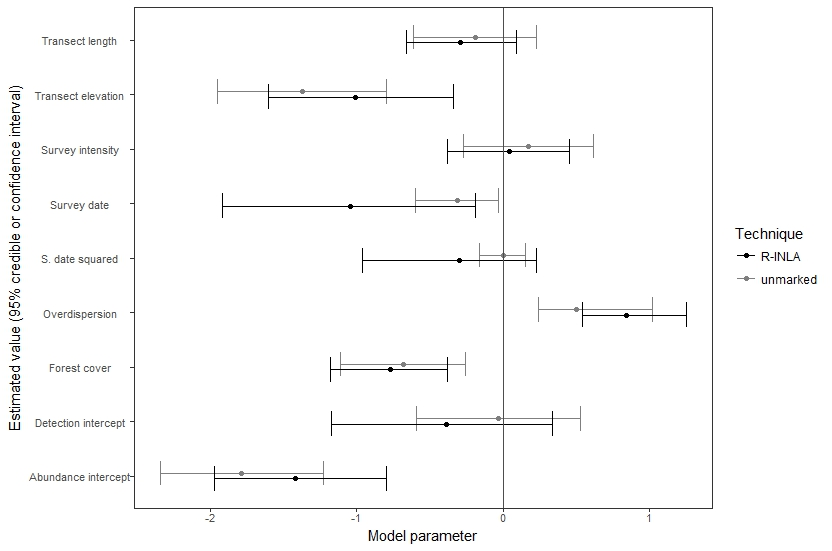
\includegraphics[width=\linewidth]{fig3.jpeg}
  \caption{Estimates and 95\% confidence intervals from \pkg{unmarked} (gray circles and lines) and posterior means and 95\% credible intervals from \pkg{R-INLA} (black lines) from an N-mixture model of mallard duck abundance.  The \pkg{unmarked} model included site-survey covariates for survey effort and survey date, while the \pkg{R-INLA} model included site-averaged versions.  A value of zero is depicted by the vertical gray line.}
  \label{fig:fig3}
\end{figure}
%% end figure 3

%% discussion
\section[Discussion]{Discussion}
The purpose of this study was to demonstrate the use of the \pkg{R-INLA} package \citep{Rue_Martino_Lindgren_Simpson_Riebler_2013} to analyze N-mixture models and to compare performance of \pkg{R-INLA} to two other common approaches, \proglang{JAGS} \citep{Lunn_Jackson_Best_Thomas_Spiegelhalter_2012}, via the \pkg{runjags} package \citep{Denwood_2016}, which employs MCMC methods and allows Bayesian inference, and the \pkg{unmarked} package \citep{Fiske_Chandler_others_2011}, which uses Maximum Likelihood and allows Frequentist inference.

Results showed that \pkg{R-INLA} can be a complementary tool in the wildlife biologist's analytical tool kit.  Strengths of \pkg{R-INLA} include Bayesian inference, based on highly accurate approximations of posterior distributions, which are derived over 300 times faster than MCMC methods, where models are specified using a syntax that should be familiar to R users, and where data are formatted in a straightforward way with relatively few lines of code.  The straightforward model syntax and data format could help remove  barriers to adoption of N-mixture models for biologists who are not committed to learning the \proglang{BUGS} syntax.  The substantial decrease in computation time should allow a wider variety of model and variable selection techniques (e.g., cross validation and model averageing), ones that are not commonly used in an MCMC context due to practical issues related to computing time \citep{Kery_Schaub_2011}.

Limitations of \pkg{R-INLA} are mainly related to the more restricted set of N-mixture models that can be specified.  Of the approaches explored here, \proglang{BUGS}-based approaches allow users ultimate flexibility in specifying models. For example, with \proglang{JAGS}, site-survey-year covariates for detection are possible, multiple types of mixed distributions are available \citep{Joseph_Elkin_Martin_Possingham_2009,Martin_Royle_Mackenzie_Edwards_Kery_Gardner_2011}, and a variety of random effects can be specified for both $\lambda$ and $p$ \citep{Kery_Schaub_2011}.  In comparison, the current version of \pkg{R-INLA} does not handle site-survey covariates, employs only Poisson-binomial and negative binomial-binomial mixtures, and handles random effects (exchangeable, spatially and temporally structured) for $p$ only.  In cases where site-survey covariates are particularly strong and not controlled in the sampling design, \pkg{R-INLA} will not be the appropriate tool (Fig. \ref{fig:fig2}).

When compared to \pkg{unmarked}, the \pkg{R-INLA} approach is similar in regards to model syntax and data format.  The approaches are also similar in that both yield results much faster than MCMC.  The two approaches differ in that \pkg{R-INLA} is roughly 10 times faster than \pkg{unmarked}, possibly due to the different approach used to compute model likelihoods (see Appendix).  They also differ in that \pkg{unmarked} can accomodate site-survey covariates and can analyze dynamic N-mixture models \citep{Chandler_Royle_King_2011, Dail_Madsen_2011}.

In conclusion, \proglang{JAGS} (and \proglang{WinBUGS}, \proglang{OpenBUGS}), \pkg{unmarked}, and \pkg{R-INLA} all allow users to employ N-mixture models for estimating wildlife abundance while accounting for imperfect detection.  Each method has its strengths and limitations.  \pkg{R-INLA} appears to be an attractive option when survey level covariates are not essential, familiar model syntax and data format are desired, fast computing time is needed, and Bayesian inference is preferred.

%% acknowledgements
\section*{Acknowledgments}
We thank the following individuals for commenting on previous drafts of this manuscript.

%% references
\bibliography{bibliog}

%% appendix
\appendix
\section{Recursive computations of the "nmix" likelihood}
The likelihood for the simplest case is
\begin{displaymath}
    \text{Probability}(y) = \sum_{n = y}^{\infty}
    \text{Poisson}(n ; \lambda) \;\times\; \text{binomial}(y;  n, p)
\end{displaymath}
where $\text{Poisson}(n; \lambda)$ is the density for the Poisson distribution with mean $\lambda$, $\lambda^{n}\exp(-\lambda)/n!$, and $\text{binomial}(y; n, p)$ is the density for the binomial distribution
with $n$ trials and probability $p$, ${n \choose y} p^{y}(1-p)^{n-p}$. Although the likelhood can be computed directly when replacing the infinite limit with a finite value, we will demonstrate here that we
can easily evaluate it using a recursive algorithm that is both faster and more numerical stable. The same idea is also applicable to the negative binomial case, and the case where we have replicated observations of the same $n$. We leave it to the reader to derive these straight forward extensions.

The key observation is that both the Poisson and the binomial distribution can be evaluated recursively in $n$,
\begin{displaymath}
    \text{Poisson}(n; \lambda) = \text{Poisson}(n-1; \lambda) \frac{\lambda}{n}
\end{displaymath}
and
\begin{displaymath}
    \text{binomial}(y; n, p) = \text{binomial}(y; n-1, p) \frac{n}{n-y}(1-p),
\end{displaymath}
and then also for the Poisson-binomial product
\begin{displaymath}
    \text{Poisson}(n ; \lambda) \; \text{binomial}(y;  n, p)
    =
    \text{Poisson}(n-1; \lambda) \; \text{binomial}(y; n-1, p)
    \frac{\lambda}{n-y}(1-p).
\end{displaymath}
If we define $f_i = \lambda(1-p)/i$ for $i=1, 2, \ldots$, we can make use of this recursive form to express the likelihood with a finite upper limit as
\begin{eqnarray}
    \text{Prob}(y) &=& \sum_{n = y}^{n_{\text{max}}}
                       \text{Poisson}(n ; \lambda)\;
                      \text{binomial}(y;  n, p) \nonumber\\
                   &=& \text{Poisson}(y; \lambda)\; \text{binomial}(y; y, p)
                       \Big\{ 1 + f_1 + f_1f_2 +
                    \ldots
                      +f_1\cdots f_{n_\text{max}}
                       \Big\} \nonumber\\
                   &=& \text{Poisson}(y; \lambda)\; \text{binomial}(y; y, p)
                       \Big\{ 1 + f_1(1+f_2(1+f_3(1+ \dots)))\Big\}\nonumber
\end{eqnarray}
The log-liklihood can then evaluated using the following simple \proglang{R}-code
\begin{Code}
R> fac <- 1; ff <- lambda * (1-p)
R> for(i in (n.max - y):1){
+    fac <- 1 + fac * ff / i
+  } 
R> log.L <- dpois(y, lambda, log = TRUE) + dbinom(y, y, p, log = TRUE) + 
+           log(fac)
\end{Code}
Since this evaluation is recursive in decreasing $n$, we have to chose the upper limit $n_\text{max}$ up-front, for example as an integer larger than $y$ so that $\frac{\lambda (1-p)}{n_\text{max}-y}$ is small. Note that we are computing \texttt{fac} starting with the smallest contributions, which are more numerically stable.


\end{document}
% %%%%%%%%%%%%%%%%%%%%%%%%%%%%%%%%%%%%%%%%%%%%%%%%%%%%%%%%%%%%%%%%%%%%%%%%%%%%%%


